% v13_pipeline_paper.tex — Multi-Fidelity Inference Pipeline for Electrochemical Kinetics
% Self-contained LaTeX document
\documentclass[11pt,a4paper]{article}

% ── Geometry ──
\usepackage[margin=1in]{geometry}

% ── Math ──
\usepackage{amsmath,amssymb,amsthm}

% ── Tables ──
\usepackage{booktabs,multirow,array}

% ── Figures & Floats ──
\usepackage{graphicx,float}

% ── Units ──
\usepackage{siunitx}
\sisetup{per-mode=symbol, exponent-product=\cdot}
\DeclareSIUnit{\molar}{M}

% ── Colors ──
\usepackage[dvipsnames]{xcolor}

% ── TikZ ──
\usepackage{tikz}
\usetikzlibrary{arrows.meta,positioning,decorations.pathreplacing,calc,fit,shapes.geometric}

% ── Plots ──
\usepackage{pgfplots}
\pgfplotsset{compat=1.18}

% ── Algorithms ──
\usepackage[ruled,vlined,linesnumbered]{algorithm2e}

% ── Code listings (minimal) ──
\usepackage{listings}
\lstset{
  basicstyle=\ttfamily\small,
  keywordstyle=\color{blue},
  commentstyle=\color{gray},
  frame=single,
  breaklines=true,
}

% ── References ──
\usepackage{hyperref}
\hypersetup{colorlinks=true, linkcolor=RoyalBlue, citecolor=ForestGreen, urlcolor=Maroon}
\usepackage[capitalise,noabbrev]{cleveref}

% ── Custom commands ──
\newcommand{\R}{\mathbb{R}}
\newcommand{\vect}[1]{\boldsymbol{#1}}
\newcommand{\dd}{\mathrm{d}}
\newcommand{\pder}[2]{\frac{\partial #1}{\partial #2}}
\newcommand{\abs}[1]{\left\lvert #1 \right\rvert}
\newcommand{\norm}[1]{\left\lVert #1 \right\rVert}
\newcommand{\kzero}{k_0}
\newcommand{\Jobj}{\mathcal{J}}
\DeclareMathOperator*{\argmin}{arg\,min}

% ── Title ──
\title{Multi-Fidelity Inference of Electrochemical Kinetics:\\
A Surrogate-Accelerated PDE-Constrained Optimization Pipeline}
\author{Jake Weinstein}
\date{March 2026}

\begin{document}
\maketitle

\begin{abstract}
We present a multi-fidelity inference pipeline for recovering four
Butler--Volmer kinetic parameters governing a two-reaction oxygen reduction
mechanism from noisy current--voltage measurements. The pipeline combines
neural-network ensemble surrogates for rapid global exploration with
PDE-constrained optimization on a Poisson--Nernst--Planck--Butler--Volmer
forward model for high-accuracy refinement. A seven-phase architecture
(five surrogate phases followed by two PDE phases) achieves
$< 5.3\%$ error on all four parameters simultaneously from data
corrupted with $2\%$ Gaussian noise, overcoming a persistent
$k_{0,1}$--$k_{0,2}$ anti-correlation that makes joint recovery
of both rate constants challenging.
The key architectural insight is a continuation strategy: a shallow-voltage
PDE phase selects the correct optimization basin before a full-cathodic
PDE phase performs final refinement. Surrogate phases contribute only
$2\%$ of total compute cost yet provide essential warm-starting that
reduces PDE phase wall-clock time by $30\%$.
\end{abstract}

\tableofcontents
\newpage

%==========================================================================
\section{Introduction}\label{sec:intro}
%==========================================================================

Electrochemical kinetics govern the performance of fuel cells, batteries,
and electrolyzers. Accurate determination of kinetic rate constants and
charge-transfer coefficients is essential for rational catalyst design and
predictive modeling. The oxygen reduction reaction (ORR) on rotating disk
electrodes (RDEs) is a canonical test system, with well-defined mass
transport that enables isolation of kinetic parameters from measured
current--voltage (I--V) curves.

\paragraph{The inverse problem.}
We consider a two-reaction ORR mechanism:
\begin{align}
  \text{R}_1&: \quad \mathrm{O_2} + 2\mathrm{H^+} + 2e^- \to
    \mathrm{H_2O_2}, \label{eq:R1}\\
  \text{R}_2&: \quad \mathrm{H_2O_2} + 2\mathrm{H^+} + 2e^- \to
    2\mathrm{H_2O}. \label{eq:R2}
\end{align}
Given noisy I--V measurements, we seek four kinetic parameters:
the heterogeneous rate constants $\kzero^{(1)}$, $\kzero^{(2)}$ and the
cathodic charge-transfer coefficients $\alpha_1$, $\alpha_2$.

\paragraph{Challenge.}
The rate constant $\kzero^{(2)}$ is approximately $24\times$ smaller than
$\kzero^{(1)}$, so Reaction~2's contribution to total current is weak at
moderate overpotentials. Its signal is buried in measurement noise and
obscured by a strong anti-correlation between $\kzero^{(1)}$ and
$\kzero^{(2)}$: improving one at the expense of the other can reduce the
objective without improving physical accuracy.

\paragraph{Contribution.}
We introduce a seven-phase multi-fidelity pipeline that achieves
$< 5.3\%$ maximum error across all four parameters. The architecture
comprises:
\begin{enumerate}
  \item Five surrogate phases using a neural-network ensemble for global
        exploration (cascade, multi-start, and joint optimization),
  \item Two PDE-constrained optimization phases that exploit the full
        physics of the Poisson--Nernst--Planck system with Butler--Volmer
        boundary conditions.
\end{enumerate}
The key insight is that a shallow-voltage PDE phase (P1) serves as a
\emph{basin selector} for the full-cathodic PDE phase (P2), analogous to
a continuation method in nonlinear optimization.

\paragraph{Outline.}
\Cref{sec:setup} defines the electrochemical system and governing equations.
\Cref{sec:forward} describes the finite-element forward solver.
\Cref{sec:inverse} formulates the inverse problem.
\Cref{sec:surrogate} presents the surrogate models.
\Cref{sec:pipeline} details the seven-phase pipeline architecture.
\Cref{sec:results} reports numerical results.
\Cref{sec:optimizations} discusses computational optimizations.
\Cref{sec:discussion} provides analysis and context.
\Cref{sec:conclusions} concludes.

%==========================================================================
\section{Problem Setup}\label{sec:setup}
%==========================================================================

\subsection{Electrochemical System}\label{sec:system}

We model oxygen reduction on a rotating disk electrode in acidic
electrolyte (pH~4, $\SI{0.1}{\molar}$ $\mathrm{HClO_4}$). The ORR
proceeds via the two-electron pathway \eqref{eq:R1}--\eqref{eq:R2},
producing hydrogen peroxide as an intermediate. Four ionic species
participate:

\begin{table}[H]
\centering
\caption{Species definitions for the four-species charged system.}
\label{tab:species}
\begin{tabular}{clcccc}
\toprule
Index $i$ & Species & Charge $z_i$ & $D_i$ (\si{\metre\squared\per\second})
  & $c_i^{\mathrm{bulk}}$ (\si{\mol\per\metre\cubed})
  & $\hat{c}_i^0$ \\
\midrule
0 & $\mathrm{O_2}$      &  0  & $1.90 \times 10^{-9}$ & 0.5   & 1.0 \\
1 & $\mathrm{H_2O_2}$   &  0  & $1.60 \times 10^{-9}$ & 0.0   & 0.0 \\
2 & $\mathrm{H^+}$      & $+1$ & $9.311\times 10^{-9}$ & 100.0 & 0.2 \\
3 & $\mathrm{ClO_4^-}$  & $-1$ & $1.792\times 10^{-9}$ & 100.0 & 0.2 \\
\bottomrule
\end{tabular}
\end{table}

Charge neutrality is maintained: $[\mathrm{H^+}] = [\mathrm{ClO_4^-}] =
\SI{0.1}{\molar}$. The physical constants are drawn from the Mangan2025
catalysis study and are listed in \cref{tab:constants}.

\begin{table}[H]
\centering
\caption{Physical constants and kinetic parameters.}
\label{tab:constants}
\begin{tabular}{llll}
\toprule
Symbol & Description & Value & Unit \\
\midrule
$F$ & Faraday constant & $96{,}485.33$ & \si{\coulomb\per\mol} \\
$R$ & Gas constant & $8.3145$ & \si{\joule\per\mol\per\kelvin} \\
$T$ & Temperature & $298.15$ & \si{\kelvin} \\
$V_T$ & Thermal voltage $RT/F$ & $0.02569$ & \si{\volt} \\
$\varepsilon_r$ & Relative permittivity (water) & $78.5$ & --- \\
$\varepsilon_0$ & Vacuum permittivity & $8.854\times10^{-12}$
  & \si{\farad\per\metre} \\
$n_e$ & Electrons per reaction & 2 & --- \\
\midrule
$\kzero^{(1)}$ & Rate constant, R$_1$ & $2.4\times10^{-8}$
  & \si{\metre\per\second} \\
$\kzero^{(2)}$ & Rate constant, R$_2$ & $1.0\times10^{-9}$
  & \si{\metre\per\second} \\
$\alpha_1$ & Transfer coefficient, R$_1$ & $0.627$ & --- \\
$\alpha_2$ & Transfer coefficient, R$_2$ & $0.500$ & --- \\
\bottomrule
\end{tabular}
\end{table}

\subsection{Governing Equations}\label{sec:governing}

The species concentrations $c_i(\vect{x},t)$ and electric potential
$\phi(\vect{x},t)$ satisfy the coupled Poisson--Nernst--Planck (PNP)
system. In nondimensional form:

\paragraph{Nernst--Planck transport.}
For each species $i = 0,\ldots, N_s-1$:
\begin{equation}\label{eq:NP}
  \pder{\hat{c}_i}{\hat{t}} = \nabla \cdot \bigl[
    \hat{D}_i\bigl( \nabla \hat{c}_i
    + z_i\, \hat{c}_i\, \nabla\hat{\phi}
    + \hat{c}_i\, \nabla \mu_{\mathrm{steric}} \bigr) \bigr],
\end{equation}
where $\hat{D}_i = D_i / D_{\mathrm{ref}}$ is the dimensionless
diffusivity and the steric (Bikerman) chemical potential is
\begin{equation}\label{eq:steric}
  \mu_{\mathrm{steric}} = \ln\!\bigl(1 - \textstyle\sum_j a_j \hat{c}_j\bigr),
\end{equation}
with $a_j = 0.01$ the steric parameter for all species.

\paragraph{Poisson equation.}
\begin{equation}\label{eq:Poisson}
  -\hat{\varepsilon}\, \nabla^2 \hat{\phi}
  = \sum_{i=0}^{N_s-1} z_i\, \hat{c}_i,
\end{equation}
where $\hat{\varepsilon} = (\lambda_D / L_{\mathrm{ref}})^2$ is the
squared Debye-to-domain length ratio.

\paragraph{Butler--Volmer kinetics.}
At the electrode surface, the flux of species $i$ due to reaction $j$ is:
\begin{equation}\label{eq:BV}
  \mathcal{R}_j = \hat{k}_0^{(j)} \Bigl[
    \hat{c}_{\mathrm{cat},j}\, \exp\!\bigl(-\alpha_j\, \hat{\eta}\bigr)
    - \hat{c}_{\mathrm{ref},j}\, \exp\!\bigl((1-\alpha_j)\,\hat{\eta}\bigr)
  \Bigr],
\end{equation}
where $\hat{\eta} = (\phi_{\mathrm{applied}} - E_{\mathrm{eq}})/V_T$ is
the dimensionless overpotential, $\hat{c}_{\mathrm{cat},j}$ is the
surface concentration of the cathodic reactant, and $\hat{c}_{\mathrm{ref},j}$
is a reference concentration for the anodic branch. Reaction~2 is
irreversible (no anodic term). The net flux boundary condition for
species $i$ on the electrode is:
\begin{equation}\label{eq:BV_flux}
  -\hat{D}_i\,\nabla \hat{c}_i \cdot \vect{n}
  = \sum_j s_{ij}\, \mathcal{R}_j,
\end{equation}
where $s_{ij}$ is the stoichiometric coefficient of species $i$ in
reaction $j$ (see \cref{tab:stoichiometry}).

\begin{table}[H]
\centering
\caption{Stoichiometric coefficients $s_{ij}$ for the two-reaction mechanism.}
\label{tab:stoichiometry}
\begin{tabular}{lrrrr}
\toprule
& $\mathrm{O_2}$ & $\mathrm{H_2O_2}$ & $\mathrm{H^+}$ & $\mathrm{ClO_4^-}$ \\
\midrule
R$_1$: $\mathrm{O_2} \to \mathrm{H_2O_2}$ & $-1$ & $+1$ & $-2$ & $0$ \\
R$_2$: $\mathrm{H_2O_2} \to \mathrm{H_2O}$ & $0$ & $-1$ & $-2$ & $0$ \\
\bottomrule
\end{tabular}
\end{table}

\subsection{Nondimensionalization}\label{sec:nondim}

We introduce reference scales to obtain the dimensionless system
\eqref{eq:NP}--\eqref{eq:Poisson}. The reference quantities and derived
scales are listed in \cref{tab:scales}.

\begin{table}[H]
\centering
\caption{Reference scales and derived nondimensional groups.}
\label{tab:scales}
\begin{tabular}{llll}
\toprule
Scale & Symbol & Expression & Typical value \\
\midrule
Length & $L_{\mathrm{ref}}$ & Domain height & $\SI{100}{\micro\metre}$ \\
Diffusivity & $D_{\mathrm{ref}}$ & $D_{\mathrm{O_2}}$ & $\SI{1.9e-9}{\metre\squared\per\second}$ \\
Concentration & $c_{\mathrm{ref}}$ & $c^{\mathrm{bulk}}_{\mathrm{O_2}}$ & $\SI{0.5}{\mol\per\metre\cubed}$ \\
Potential & $V_T$ & $RT/F$ & $\SI{25.69}{\milli\volt}$ \\
\midrule
Time & $t_{\mathrm{ref}}$ & $L_{\mathrm{ref}}^2 / D_{\mathrm{ref}}$ & $\SI{5.26}{\second}$ \\
Velocity & $\kappa_{\mathrm{ref}}$ & $D_{\mathrm{ref}} / L_{\mathrm{ref}}$ & $\SI{1.9e-5}{\metre\per\second}$ \\
Current density & $I_{\mathrm{ref}}$ & $n_e F D_{\mathrm{ref}} c_{\mathrm{ref}} / L_{\mathrm{ref}}$ & $\SI{1.83}{\milli\ampere\per\centi\metre\squared}$ \\
Debye length & $\lambda_D$ & $\sqrt{\varepsilon_r \varepsilon_0 V_T / (F\, c_{\mathrm{bulk}})}$ & $\SI{\sim 3}{\nano\metre}$ \\
Debye ratio & $\hat{\varepsilon}$ & $(\lambda_D / L_{\mathrm{ref}})^2$ & $\sim 9\times 10^{-8}$ \\
\bottomrule
\end{tabular}
\end{table}

The rate constants are nondimensionalized as
$\hat{k}_0^{(j)} = k_0^{(j)} / \kappa_{\mathrm{ref}}$, giving
$\hat{k}_0^{(1)} \approx 1.26$ and $\hat{k}_0^{(2)} \approx 0.053$.
The current density scale $I_{\mathrm{ref}}$ converts dimensionless
species flux to physical units via
$I_{\mathrm{CD}} = I_{\mathrm{ref}} \times (\text{dimensionless flux})$.

\subsection{Domain and Boundary Conditions}\label{sec:domain}

The computational domain is a two-dimensional rectangle
$\Omega = [0, L_x] \times [0, L_y]$ with graded mesh
(see \cref{sec:mesh} for discretization details). The boundary is
partitioned as shown in \cref{fig:domain}.

\begin{figure}[H]
\centering
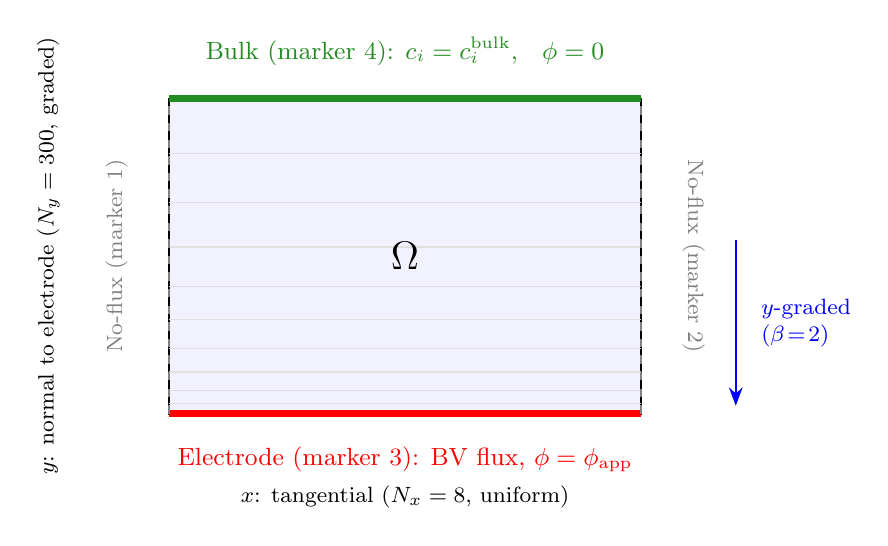
\begin{tikzpicture}[>=Stealth]
  % Domain — diffusion layer above RDE electrode
  % Bottom = electrode (y=0), Top = bulk (y=1)
  % Left/Right = no-flux symmetry
  \fill[blue!5] (0,0) rectangle (6,4);
  \draw[thick] (0,0) rectangle (6,4);

  % Mesh grading lines (drawn first, behind everything)
  \foreach \i in {1,...,10}{
    \pgfmathsetmacro{\yy}{4.0*((\i/11)^2)}
    \draw[black!12] (0,\yy) -- (6,\yy);
  }

  % Boundary coloring (on top of mesh lines)
  \draw[red, line width=2.5pt] (0,0) -- (6,0);           % electrode
  \draw[ForestGreen, line width=2.5pt] (0,4) -- (6,4);   % bulk
  \draw[gray, thick, dashed] (0,0) -- (0,4);              % no-flux L
  \draw[gray, thick, dashed] (6,0) -- (6,4);              % no-flux R

  % --- Labels (well-separated) ---

  % Bottom: electrode
  \node[red, font=\small, anchor=north] at (3,-0.3)
    {Electrode (marker 3): BV flux, $\phi = \phi_{\mathrm{app}}$};

  % Top: bulk
  \node[ForestGreen, font=\small, anchor=south] at (3,4.3)
    {Bulk (marker 4): $c_i = c_i^{\mathrm{bulk}}$, \; $\phi = 0$};

  % Left side
  \node[gray, font=\footnotesize, rotate=90, anchor=south] at (-0.4, 2)
    {No-flux (marker 1)};

  % Right side
  \node[gray, font=\footnotesize, rotate=-90, anchor=south] at (6.4, 2)
    {No-flux (marker 2)};

  % --- Interior annotations ---

  % Domain label
  \node[font=\Large] at (3, 2) {$\Omega$};

  % --- Grading annotation (far right, no overlap with marker 2 label) ---
  \draw[<-, thick, blue] (7.2, 0.1) -- (7.2, 2.2);
  \node[blue, font=\footnotesize, anchor=west, align=left] at (7.4, 1.15)
    {$y$-graded\\$(\beta\!=\!2)$};

  % --- Axis labels along edges ---
  \node[font=\footnotesize, anchor=north] at (3, -0.8)
    {$x$: tangential ($N_x = 8$, uniform)};
  \node[font=\footnotesize, rotate=90, anchor=north] at (-1.8, 2)
    {$y$: normal to electrode ($N_y = 300$, graded)};
\end{tikzpicture}
\caption{Computational domain representing the diffusion layer above a
  rotating disk electrode. The bottom boundary (marker~3) is the electrode
  surface with Butler--Volmer flux boundary conditions; the top boundary
  (marker~4) imposes bulk Dirichlet concentrations and ground potential;
  left and right boundaries (markers~1,2) are no-flux (symmetry).
  The mesh is graded in $y$ with $\beta=2$, clustering elements near
  the electrode to resolve steep concentration gradients and the Debye
  screening layer.}
\label{fig:domain}
\end{figure}

\subsection{Observables}\label{sec:observables}

Two observables are extracted from each forward solve at overpotential
$\eta$:

\paragraph{Current density $I_{\mathrm{CD}}$.}
The total Faradaic current density, integrated over the electrode surface:
\begin{equation}\label{eq:ICD}
  I_{\mathrm{CD}}(\eta) = I_{\mathrm{ref}} \sum_j
  \int_{\Gamma_{\mathrm{elec}}} \mathcal{R}_j \, \dd s.
\end{equation}
This captures the overall reduction current (dominated by R$_1$).

\paragraph{Peroxide current $I_{\mathrm{PC}}$.}
The current associated with net peroxide production:
\begin{equation}\label{eq:IPC}
  I_{\mathrm{PC}}(\eta) = I_{\mathrm{ref}}
  \int_{\Gamma_{\mathrm{elec}}}
  \bigl(\mathcal{R}_1 - \mathcal{R}_2\bigr) \,\dd s.
\end{equation}
Since $\mathcal{R}_1$ produces $\mathrm{H_2O_2}$ and $\mathcal{R}_2$
consumes it, $I_{\mathrm{PC}}$ is sensitive to the ratio
$\kzero^{(2)}/\kzero^{(1)}$ and is essential for identifiability of the
four-parameter system. Without $I_{\mathrm{PC}}$, the $\kzero^{(1)}$--$\kzero^{(2)}$
pair is poorly determined.

\paragraph{Experimental measurement.}
Both observables are accessible in a single experiment using a
rotating ring-disk electrode (RRDE)~\cite{ruggiero2022}.
An RRDE consists of a small \emph{disk} (the catalyst surface)
surrounded by a concentric \emph{ring}, both submerged in solution
and spinning.  The disk voltage is swept while its current is
recorded---this is $I_{\mathrm{CD}}$, capturing the total
electrochemical activity (both O$_2 \to$ H$_2$O$_2$ and
H$_2$O$_2 \to$ H$_2$O).  The ring is held at a fixed potential
that oxidizes any H$_2$O$_2$ drifting outward from the disk; its
current, after dividing by a known geometric correction factor
(collection efficiency~$N$), gives $I_{\mathrm{PC}}$.
Sweeping the disk potential therefore produces both I--V curves
simultaneously---exactly the pair of observables the inverse problem
needs to disentangle the two reaction rate constants.
This experimental grounding motivates the two-observable objective
function~\eqref{eq:objective}: the disk current constrains the dominant
reaction (R$_1$) while the ring current constrains the secondary
reaction (R$_2$).

%==========================================================================
\section{Forward Solver}\label{sec:forward}
%==========================================================================

The forward solver computes steady-state solutions of the PNP--BV system
\eqref{eq:NP}--\eqref{eq:BV_flux} at a sequence of overpotentials,
producing I--V curves for both observables. It is implemented in
Firedrake, a finite-element framework built on PETSc.

\subsection{Finite Element Discretization}\label{sec:mesh}

\paragraph{Mesh.}
The domain is discretized with a structured rectangle mesh:
$N_x = 8$ elements in the tangential direction (uniform) and
$N_y = 300$ elements in the normal direction with power-law grading:
\begin{equation}\label{eq:grading}
  y_k = \left(\frac{k}{N_y}\right)^{\!\beta}, \qquad k=0,\ldots,N_y,
\end{equation}
with $\beta = 2$. This clusters nodes near the electrode ($y=0$) to
resolve thin boundary layers and the Debye screening region.

\paragraph{Function space.}
We use a mixed function space consisting of $N_s + 1$ copies of
continuous Galerkin elements of degree 1 (CG$_1$):
\begin{equation}
  W = \underbrace{V_h \times \cdots \times V_h}_{N_s \text{ species}}
    \times V_h^{(\phi)}, \qquad
  V_h = \mathrm{CG}_1(\mathcal{T}_h).
\end{equation}
The solution vector $U = (c_0, c_1, \ldots, c_{N_s-1}, \phi) \in W$
combines all species concentrations and the electric potential.

\paragraph{Weak form.}
The variational formulation for test function $v = (v_0,\ldots,v_{N_s-1},w)
\in W$ reads:
\begin{multline}\label{eq:weak}
  F(U;v) = \sum_{i=0}^{N_s-1} \int_\Omega \frac{c_i - c_i^{\mathrm{old}}}{\Delta t}\, v_i \,\dd x
  + \sum_{i=0}^{N_s-1} \int_\Omega \hat{D}_i \bigl(
    \nabla c_i + z_i\, c_i \nabla\phi + c_i \nabla\mu_{\mathrm{steric}}
  \bigr) \cdot \nabla v_i \,\dd x \\
  - \sum_{i,j} s_{ij} \int_{\Gamma_{\mathrm{elec}}} \mathcal{R}_j \, v_i \,\dd s
  + \hat{\varepsilon} \int_\Omega \nabla\phi \cdot \nabla w \,\dd x
  - \int_\Omega \Bigl(\sum_i z_i c_i\Bigr) w \,\dd x = 0.
\end{multline}
The system is solved with Newton's method using PETSc's SNES
(Scalable Nonlinear Equations Solvers) with MUMPS direct factorization.

\subsection{Pseudo-Transient Continuation}\label{sec:ptc}

Direct Newton iteration on the steady-state residual often diverges for
large overpotentials due to the exponential nonlinearity of the
Butler--Volmer terms. We embed the steady-state problem in fictitious
time-stepping:
\begin{equation}\label{eq:ptc}
  \frac{1}{\Delta t_{\mathrm{ptc}}} M(U^{n+1} - U^n) + F(U^{n+1}) = 0,
\end{equation}
where $M$ is the mass matrix. As $\Delta t_{\mathrm{ptc}} \to \infty$,
\eqref{eq:ptc} reduces to the steady-state problem $F(U) = 0$.

\paragraph{Adaptive time-stepping.}
The pseudo-time step is adapted using the Switched Evolution Relaxation
(SER) strategy:
\begin{equation}\label{eq:SER}
  \Delta t_{\mathrm{ptc}}^{n+1}
  = \Delta t_{\mathrm{ptc}}^n \cdot
    \frac{\norm{r^{n-1}}}{\max(\norm{U^n - U^{n-1}},\, 10^{-30})}
    \cdot \gamma,
\end{equation}
where $\gamma = 1.5$ is the growth factor and the step is clamped at
$\Delta t_{\max} = 10^6$. The initial step is
$\Delta t_0 = 0.01$, which provides Picard-like regularization. Steady
state is declared when 4 consecutive steps satisfy
$\norm{U^{n+1}-U^n}/\norm{U^n} < 10^{-5}$.

\subsection{Voltage Sweep via Continuation}\label{sec:vsweep}

An I--V curve requires solving at multiple overpotentials
$\eta_1, \eta_2, \ldots, \eta_M$. Rather than solving each independently,
we use \emph{voltage continuation}: the converged solution at $\eta_k$ is
used as the initial condition for $\eta_{k+1}$, dramatically reducing the
number of pseudo-transient steps required.

\begin{figure}[H]
\centering
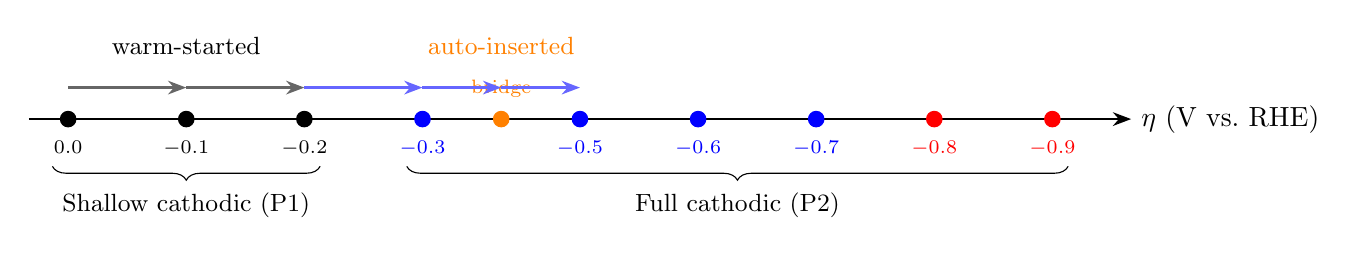
\begin{tikzpicture}[>=Stealth, scale=1.0]
  % Axis
  \draw[->, thick] (0,0) -- (14,0) node[right] {$\eta$ (V vs.\ RHE)};

  % Shallow cathodic points (black)
  \foreach \x/\lab in {0.5/$0.0$, 2.0/$-0.1$, 3.5/$-0.2$}{
    \fill[black] (\x, 0) circle (3pt);
    \node[below, font=\scriptsize] at (\x, -0.15) {\lab};
  }
  % Full cathodic points (blue)
  \foreach \x/\lab in {5.0/$-0.3$, 7.0/$-0.5$, 8.5/$-0.6$, 10.0/$-0.7$}{
    \fill[blue] (\x, 0) circle (3pt);
    \node[below, font=\scriptsize, blue] at (\x, -0.15) {\lab};
  }
  % Deep cathodic points (red)
  \foreach \x/\lab in {11.5/$-0.8$, 13.0/$-0.9$}{
    \fill[red] (\x, 0) circle (3pt);
    \node[below, font=\scriptsize, red] at (\x, -0.15) {\lab};
  }

  % Bridge point
  \fill[orange] (6.0, 0) circle (3pt);
  \node[above, font=\scriptsize, orange] at (6.0, 0.15) {bridge};

  % Arrows showing continuation
  \draw[->, thick, black!60] (0.5, 0.4) -- (2.0, 0.4);
  \draw[->, thick, black!60] (2.0, 0.4) -- (3.5, 0.4);
  \draw[->, thick, blue!60] (3.5, 0.4) -- (5.0, 0.4);
  \draw[->, thick, blue!60] (5.0, 0.4) -- (6.0, 0.4);
  \draw[->, thick, blue!60] (6.0, 0.4) -- (7.0, 0.4);

  % Labels
  \draw[decorate, decoration={brace, amplitude=5pt, mirror}]
    (0.3,-0.6) -- (3.7,-0.6) node[midway, below=6pt, font=\small]
    {Shallow cathodic (P1)};
  \draw[decorate, decoration={brace, amplitude=5pt, mirror}]
    (4.8,-0.6) -- (13.2,-0.6) node[midway, below=6pt, font=\small]
    {Full cathodic (P2)};

  % Phase labels
  \node[above, font=\small, black] at (2.0, 0.7) {warm-started};
  \node[above, font=\small, orange] at (6.0, 0.7)
    {auto-inserted};
\end{tikzpicture}
\caption{Voltage continuation strategy. Solutions propagate left to right
  along the $\eta$-axis. Bridge points (orange) are auto-inserted when
  the gap between consecutive targets exceeds a threshold. The shallow
  cathodic range (P1, 10 points) provides warm-starting for the full
  cathodic range (P2, 15 points).}
\label{fig:continuation}
\end{figure}

\paragraph{Bridge point auto-insertion.}
When the gap between consecutive voltage points exceeds a threshold,
intermediate \emph{bridge points} are automatically inserted to maintain
continuity of the solution manifold. These bridge points are solved but
not included in the output I--V curve.

\paragraph{Mixed-sign sweep ordering.}
Positive and negative overpotentials are handled by sweeping from
equilibrium ($\eta=0$) outward in both directions, reusing the
equilibrium solution as the branch point.

\paragraph{Predictor warm-starts.}
Between voltage points in the continuation sweep, we use 3-point
quadratic Lagrange interpolation to predict the solution at the next
voltage:
\begin{equation}\label{eq:predictor}
  U_{\text{pred}}(\eta_{k+1}) \approx \sum_{j=0}^{2}
    U(\eta_{k-j}) \prod_{\substack{m=0\\m\neq j}}^{2}
    \frac{\eta_{k+1} - \eta_{k-m}}{\eta_{k-j} - \eta_{k-m}}.
\end{equation}
The predictor is validated: if the predicted concentration is negative or
the potential exceeds physical bounds, the predictor is rejected and the
previous converged solution is used instead.

\subsection{Charge Continuation}\label{sec:charge_cont}

For charged species, the Debye parameter
$\hat{\varepsilon} = (\lambda_D / L_{\mathrm{ref}})^2 \approx 9\times10^{-8}$
introduces extreme stiffness in the Poisson equation. We employ a
two-phase charge continuation strategy:

\begin{enumerate}
  \item \textbf{Phase~1 (Neutral sweep):} Set all charges $z_i = 0$,
    effectively decoupling the Poisson equation. The system reduces to
    pure diffusion-reaction, which is much easier to solve. Sweep the
    full voltage range to obtain approximate concentration profiles.
  \item \textbf{Phase~2 (Charge ramping):} At the target overpotential,
    gradually restore the physical charges by ramping a factor
    $\zeta \in [0, 1]$:
    \begin{equation}
      z_i^{(\zeta)} = \zeta \cdot z_i^{\mathrm{phys}},
      \qquad \zeta = 0, 0.1, 0.2, \ldots, 1.0.
    \end{equation}
    The Poisson coupling strengthens progressively, with each step
    warm-started from the previous converged solution.
\end{enumerate}

\subsection{Convergence Safeguards}\label{sec:safeguards}

Several safeguards ensure robust convergence:

\begin{itemize}
  \item \textbf{Exponent clipping:} The Butler--Volmer exponent
    $\alpha_j \hat{\eta}$ is clipped to $[-50, +50]$ to prevent floating-point
    overflow ($e^{50} \approx 5.2\times10^{21}$).
  \item \textbf{Concentration floor:} Surface concentrations in the BV
    expression are regularized via
    $\hat{c}_{\mathrm{surf}} = \max(\hat{c}_i, \epsilon_c)$ with
    $\epsilon_c = 10^{-8}$, preventing $\log(0)$ in steric terms.
  \item \textbf{MUMPS auto-scaling:} The MUMPS direct solver is configured
    with \texttt{icntl(8)=77} for automatic matrix scaling, critical for
    the ill-conditioned systems arising from charged electrolytes.
  \item \textbf{Conservative line search:} The Newton line search maximum
    step is limited to $\lambda_{\max} = 0.5$, preventing overshoot in
    the highly nonlinear regime.
  \item \textbf{Jacobian lag:} The Jacobian is recomputed at every Newton
    step (no lagging) to maintain quadratic convergence near the solution.
\end{itemize}

The SNES configuration is summarized in \cref{tab:snes}.

\begin{table}[H]
\centering
\caption{PETSc/SNES solver configuration.}
\label{tab:snes}
\begin{tabular}{ll}
\toprule
Parameter & Value \\
\midrule
SNES type & \texttt{newtonls} \\
Max iterations & 200 (neutral) / 300 (charged) \\
Absolute tolerance & $10^{-7}$ \\
Relative tolerance & $10^{-10}$ \\
Step tolerance & $10^{-12}$ \\
Line search & \texttt{l2}, $\lambda_{\max} = 0.5$ \\
Divergence tolerance & $10^{12}$ \\
Linear solver & MUMPS direct (\texttt{preonly} + \texttt{lu}) \\
MUMPS scaling & \texttt{icntl(8)} = 77 (auto) \\
MUMPS memory & \texttt{icntl(14)} = 80 \\
\bottomrule
\end{tabular}
\end{table}


%==========================================================================
\section{The Inverse Problem}\label{sec:inverse}
%==========================================================================

\subsection{Control Variables}\label{sec:controls}

The parameter vector to be recovered is:
\begin{equation}\label{eq:theta}
  \vect{\theta} = \bigl(\log_{10} \kzero^{(1)},\;
    \log_{10} \kzero^{(2)},\; \alpha_1,\; \alpha_2 \bigr) \in \R^4.
\end{equation}
Rate constants are parameterized in log-space because they span orders of
magnitude ($\kzero^{(2)} / \kzero^{(1)} \approx 1/24$) and log-space
provides natural scaling for the optimizer.

\subsection{Objective Function}\label{sec:objective}

Given observed I--V curves $I_{\mathrm{CD}}^{\mathrm{obs}}(\eta_m)$ and
$I_{\mathrm{PC}}^{\mathrm{obs}}(\eta_m)$ at voltage points
$\{\eta_m\}_{m=1}^M$, the objective function is:
\begin{equation}\label{eq:objective}
  \Jobj(\vect{\theta}) = \frac{1}{2}\sum_{m=1}^M
    \bigl(I_{\mathrm{CD}}(\eta_m; \vect{\theta}) - I_{\mathrm{CD}}^{\mathrm{obs}}(\eta_m)\bigr)^2
  + \frac{w}{2}\sum_{m=1}^M
    \bigl(I_{\mathrm{PC}}(\eta_m; \vect{\theta}) - I_{\mathrm{PC}}^{\mathrm{obs}}(\eta_m)\bigr)^2,
\end{equation}
where $w > 0$ is a weight controlling the relative importance of
the peroxide current observable. The weight $w$ is varied across pipeline
phases to emphasize different observables (\cref{sec:cascade}).

\subsection{Gradient Computation}\label{sec:gradients}

\paragraph{PDE phases.}
For the PDE-constrained optimization phases, gradients of $\Jobj$ with
respect to $\vect{\theta}$ are computed via the adjoint method. The
forward PDE solve produces the state $U(\vect{\theta})$; two adjoint
passes (one per observable) yield the gradient components. The adjoint
equations are assembled and solved using dolfin-adjoint (pyadjoint).

The gradient in log-space follows from the chain rule:
\begin{equation}\label{eq:loggradient}
  \frac{\partial \Jobj}{\partial \log_{10} k_0^{(j)}}
  = k_0^{(j)} \ln(10) \cdot \frac{\partial \Jobj}{\partial k_0^{(j)}}.
\end{equation}

\paragraph{Surrogate phases.}
For surrogate-based optimization, gradients are approximated by central
finite differences with step size $h = 10^{-5}$:
\begin{equation}\label{eq:fd_grad}
  \frac{\partial \Jobj}{\partial \theta_i}
  \approx \frac{\Jobj(\vect{\theta} + h\,\vect{e}_i) - \Jobj(\vect{\theta} - h\,\vect{e}_i)}{2h}.
\end{equation}
Each gradient evaluation requires $2 \times 4 = 8$ surrogate predictions,
each costing $\sim\!\SI{1}{\milli\second}$.

\subsection{L-BFGS-B Optimizer}\label{sec:lbfgsb}

All optimization phases use the L-BFGS-B algorithm (limited-memory
Broyden--Fletcher--Goldfarb--Shanno with box constraints), well-suited to
this problem because:
\begin{itemize}
  \item The objective is smooth (continuous PDE solution or smooth NN
    surrogate).
  \item Box constraints enforce physical bounds on $\alpha \in [0.1, 0.9]$
    and $\log_{10} k_0 \in [-7, 0]$.
  \item The parameter dimension ($d=4$) is low, so the L-BFGS Hessian
    approximation is highly effective.
\end{itemize}

\begin{table}[H]
\centering
\caption{L-BFGS-B optimizer settings per pipeline phase.}
\label{tab:lbfgsb}
\begin{tabular}{lccc}
\toprule
Phase & \texttt{maxiter} & \texttt{ftol} & \texttt{gtol} \\
\midrule
S1 (alpha init) & 30 & $10^{-14}$ & $10^{-8}$ \\
S2 (joint) & 60 & $10^{-14}$ & $10^{-8}$ \\
S3 (cascade, per pass) & 60 / 60 / 30 & $10^{-14}$ & $10^{-8}$ \\
S4 (multistart polish) & 60 & $10^{-14}$ & $10^{-8}$ \\
P1 (PDE shallow) & 20 & $10^{-12}$ & $10^{-6}$ \\
P2 (PDE full) & 20 & $10^{-12}$ & $10^{-6}$ \\
\bottomrule
\end{tabular}
\end{table}

\subsection{The \texorpdfstring{$k_{0,2}$}{k0,2} Identifiability Challenge}\label{sec:identifiability}

The second rate constant $\kzero^{(2)}$ is the most difficult parameter
to recover for several reasons:

\begin{enumerate}
  \item \textbf{Reaction rate ratio:} At moderate overpotentials,
    $\mathcal{R}_2 \ll \mathcal{R}_1$ because $\kzero^{(2)}$ is $24\times$
    smaller. The contribution of R$_2$ to total current is marginal.
  \item \textbf{Cancellation sensitivity:} The peroxide current
    $I_{\mathrm{PC}} \propto \mathcal{R}_1 - \mathcal{R}_2$ is a
    difference of two nearly equal quantities at large $|\eta|$, making
    it sensitive to numerical errors and noise amplification.
  \item \textbf{Anti-correlation:} The optimizer can trade $\kzero^{(1)}$
    against $\kzero^{(2)}$---increasing one while decreasing the other---and
    achieve a similar total current. This manifests as an elongated valley
    in the objective landscape.
\end{enumerate}

\Cref{tab:tradeoff} documents this trade-off across pipeline versions.

\begin{table}[H]
\centering
\caption{The $\kzero^{(1)}$--$\kzero^{(2)}$ trade-off across versions.
  Prior to v13, no version achieved $< 10\%$ on both rate constants simultaneously.}
\label{tab:tradeoff}
\begin{tabular}{lcccc}
\toprule
Version & $\kzero^{(1)}$ error & $\kzero^{(2)}$ error & Sum & Max \\
\midrule
v7 (PDE only) & 10.9\% & 2.6\% & 13.5\% & 10.9\% \\
v11 P4 (RBF$\to$PDE) & 9.4\% & 0.8\% & 10.2\% & 9.4\% \\
v12 P3 (NN$\to$PDE) & 6.8\% & 11.8\% & 18.6\% & 11.8\% \\
v12 P4 (NN$\to$PDE full) & 16.6\% & 6.0\% & 22.6\% & 16.6\% \\
\midrule
\textbf{v13 P2} & \textbf{4.78\%} & \textbf{4.23\%} & \textbf{9.01\%} & \textbf{5.26\%} \\
\bottomrule
\end{tabular}
\end{table}


%==========================================================================
\section{Surrogate Models}\label{sec:surrogate}
%==========================================================================

\subsection{Training Data Generation}\label{sec:training_data}

Training samples are generated via Latin Hypercube Sampling (LHS) over
the four-dimensional parameter space:
\begin{itemize}
  \item $\log_{10}(\kzero^{(1)}) \in [-6, 0]$ \quad (log-uniform),
  \item $\log_{10}(\kzero^{(2)}) \in [-7, -1]$ \quad (log-uniform),
  \item $\alpha_1 \in [0.1, 0.9]$ \quad (uniform),
  \item $\alpha_2 \in [0.1, 0.9]$ \quad (uniform).
\end{itemize}
Each sample requires a full PDE voltage sweep producing a 22-point I--V
curve pair ($I_{\mathrm{CD}}, I_{\mathrm{PC}}$). Approximately 2000
samples are used for the NN ensemble and 445 for the RBF baseline.

\subsection{Neural Network Architecture}\label{sec:nn_arch}

We use a residual MLP (ResNet-MLP) with the architecture shown in
\cref{fig:nn_arch}.

\begin{figure}[H]
\centering
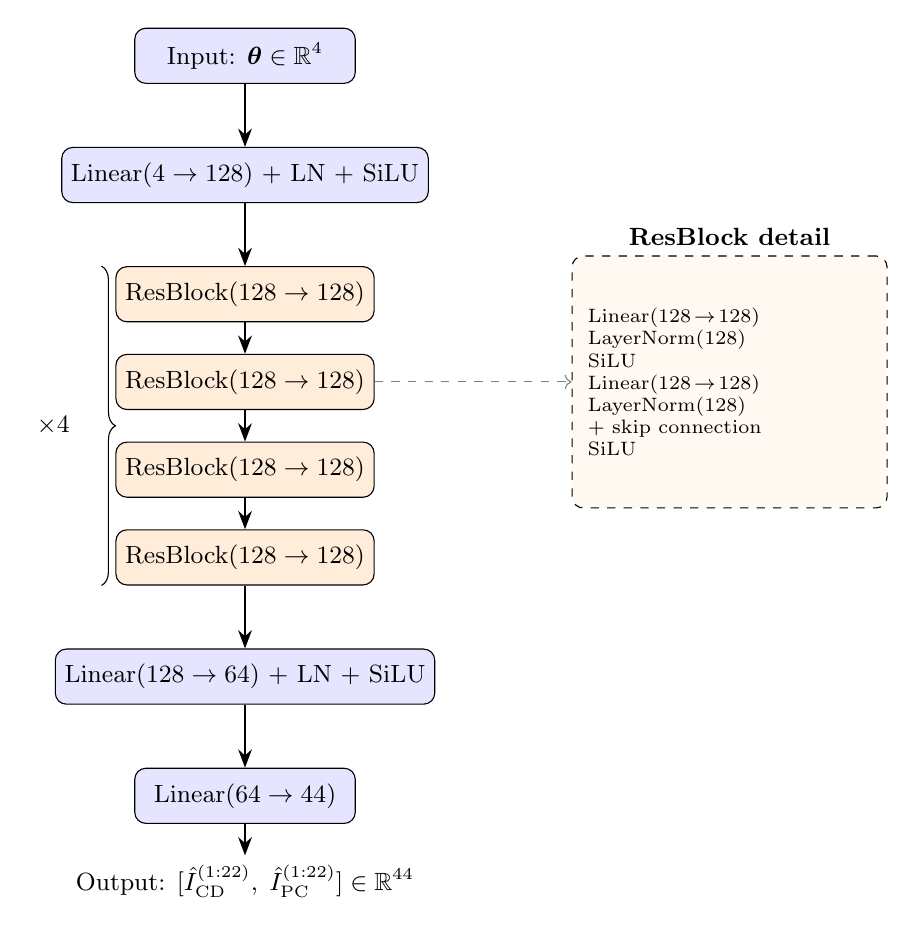
\begin{tikzpicture}[
  node distance=0.8cm,
  block/.style={draw, rounded corners, minimum width=2.8cm, minimum height=0.7cm,
    fill=blue!10, font=\small},
  resblock/.style={draw, rounded corners, minimum width=3.2cm, minimum height=0.7cm,
    fill=orange!15, font=\small},
  arrow/.style={->, >=Stealth, thick},
]
  % Input
  \node[block] (input) {Input: $\vect{\theta} \in \R^4$};

  % Input projection
  \node[block, below=of input] (proj) {Linear$(4 \to 128)$ + LN + SiLU};
  \draw[arrow] (input) -- (proj);

  % ResBlocks
  \node[resblock, below=of proj] (rb1) {ResBlock$(128 \to 128)$};
  \node[resblock, below=0.4cm of rb1] (rb2) {ResBlock$(128 \to 128)$};
  \node[resblock, below=0.4cm of rb2] (rb3) {ResBlock$(128 \to 128)$};
  \node[resblock, below=0.4cm of rb3] (rb4) {ResBlock$(128 \to 128)$};

  \draw[arrow] (proj) -- (rb1);
  \draw[arrow] (rb1) -- (rb2);
  \draw[arrow] (rb2) -- (rb3);
  \draw[arrow] (rb3) -- (rb4);

  % ResBlock detail (side box)
  \node[draw, dashed, rounded corners, right=2.5cm of rb2,
    minimum width=4cm, minimum height=3.2cm, fill=orange!5] (detail) {};
  \node[above, font=\small\bfseries] at (detail.north) {ResBlock detail};
  \node[font=\scriptsize, text width=3.6cm, align=left] at (detail.center) {
    Linear$(128\!\to\!128)$\\
    LayerNorm$(128)$\\
    SiLU\\
    Linear$(128\!\to\!128)$\\
    LayerNorm$(128)$\\
    + skip connection\\
    SiLU
  };
  \draw[->, dashed, gray] (rb2.east) -- (detail.west);

  % Output layers
  \node[block, below=of rb4] (out1) {Linear$(128 \to 64)$ + LN + SiLU};
  \node[block, below=of out1] (out2) {Linear$(64 \to 44)$};

  \draw[arrow] (rb4) -- (out1);
  \draw[arrow] (out1) -- (out2);

  % Output label
  \node[below=0.4cm of out2, font=\small] (outlabel)
    {Output: $[\hat{I}_{\mathrm{CD}}^{(1:22)},\; \hat{I}_{\mathrm{PC}}^{(1:22)}] \in \R^{44}$};
  \draw[arrow] (out2) -- (outlabel);

  % Brace for ResBlocks
  \draw[decorate, decoration={brace, amplitude=5pt}]
    ([xshift=-5pt]rb1.north west) -- ([xshift=-5pt]rb4.south west)
    node[midway, left=8pt, font=\small] {$\times 4$};
\end{tikzpicture}
\caption{ResNet-MLP architecture. Four residual blocks with LayerNorm
  and SiLU activation map the 4-parameter input to 44 outputs
  (22 current density + 22 peroxide current values). Total:
  $\sim\!145\text{K}$ parameters.}
\label{fig:nn_arch}
\end{figure}

\paragraph{Architecture details.}
The input layer projects the 4-dimensional parameter vector to a
128-dimensional hidden representation via a linear layer, LayerNorm, and
SiLU (Sigmoid Linear Unit, $\text{SiLU}(x) = x\sigma(x)$) activation.
Four residual blocks each apply two linear layers with LayerNorm and a
skip connection. The output head compresses to 64 dimensions before
a final linear layer produces the 44-dimensional output (22 voltage
points $\times$ 2 observables).

\subsection{Training Procedure}\label{sec:training}

\begin{table}[H]
\centering
\caption{Neural network training hyperparameters.}
\label{tab:nn_hyper}
\begin{tabular}{ll}
\toprule
Hyperparameter & Value \\
\midrule
Optimizer & AdamW \\
Learning rate & $10^{-3}$ \\
Weight decay & $10^{-4}$ \\
LR schedule & CosineAnnealingWarmRestarts ($T_0=500$, $T_{\mathrm{mult}}=2$, $\eta_{\min}=10^{-6}$) \\
Max epochs & 5000 \\
Early stopping patience & 500 epochs \\
Validation fraction & 15\% \\
Loss & MSE (full-batch) \\
Input normalization & Z-score ($k_0$ in $\log_{10}$ space) \\
Output normalization & Z-score (concatenated CD+PC) \\
\bottomrule
\end{tabular}
\end{table}

Training uses full-batch gradient descent with AdamW and a cosine
annealing schedule with warm restarts. The warm restart periods double
each cycle ($T_0 = 500$, $T_{\mathrm{mult}} = 2$), allowing the
optimizer to escape shallow local minima. Early stopping monitors
validation loss with a patience of 500 epochs, restoring the best model.

Input normalization applies z-score standardization after transforming
rate constants to $\log_{10}$ space. Output normalization z-scores the
concatenated 44-dimensional curve vector. Standard deviations are clamped
at $10^{-15}$ for numerical stability.

\subsection{Ensemble Construction}\label{sec:ensemble}

An ensemble of $K = 5$ independently trained networks provides both
improved predictions and uncertainty quantification:
\begin{itemize}
  \item Each member uses a different random seed for weight initialization
    and a different train/validation split (permutation-based).
  \item The ensemble prediction is the member-wise mean:
    $\bar{f}(\vect{\theta}) = \frac{1}{K}\sum_{k=1}^K f_k(\vect{\theta})$.
  \item Pointwise uncertainty is estimated by the ensemble standard
    deviation: $\sigma(\vect{\theta}) = \mathrm{std}_{k=1}^K f_k(\vect{\theta})$.
\end{itemize}

Ensembling improves over single models by averaging out individual
network biases and providing a model-free uncertainty estimate. The
ensemble spread is used diagnostically in \cref{sec:results} to explain
why $\kzero^{(2)}$ is harder to recover.

\subsection{RBF Baseline}\label{sec:rbf}

As a baseline, we fit two thin-plate spline RBF interpolants (one per
observable) using \texttt{scipy.interpolate.RBFInterpolator}:
\begin{itemize}
  \item Kernel: thin-plate spline ($r^2 \log r$),
  \item Polynomial degree: 1,
  \item Smoothing: 0 (exact interpolation),
  \item Input normalization: z-score (with $k_0$ in $\log_{10}$ space).
\end{itemize}
The RBF model is simpler (no training loop, no hyperparameters beyond
the kernel) but scales poorly with sample count ($O(N^3)$ construction)
and provides no built-in uncertainty estimate.

\subsection{Model Evaluation}\label{sec:model_eval}

Both surrogates expose a unified prediction API:
\begin{itemize}
  \item \texttt{predict($\kzero^{(1)}, \kzero^{(2)}, \alpha_1, \alpha_2$)}
    returns current density and peroxide current arrays.
  \item \texttt{predict\_batch} accepts arrays for vectorized evaluation
    (critical for the multi-start grid search).
  \item \texttt{predict\_with\_uncertainty} (ensemble only) returns mean
    and standard deviation.
\end{itemize}


%==========================================================================
\section{Inference Pipeline Architecture}\label{sec:pipeline}
%==========================================================================

\subsection{Overview}\label{sec:overview}

The v13 pipeline comprises seven phases organized in two tiers:
five surrogate-based phases (S1--S5) for rapid global exploration,
followed by two PDE-constrained phases (P1--P2) for high-accuracy
refinement. \Cref{fig:pipeline} shows the complete architecture.

\begin{figure}[H]
\centering
\resizebox{\textwidth}{!}{%
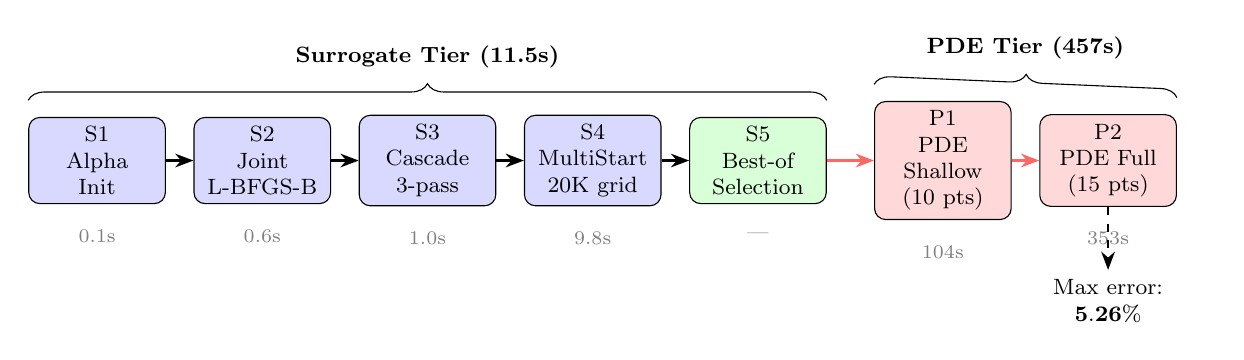
\begin{tikzpicture}[
  node distance=0.25cm and 0.35cm,
  phase/.style={draw, rounded corners, minimum width=1.7cm, minimum height=0.9cm,
    font=\footnotesize, text width=1.5cm, align=center},
  surr/.style={phase, fill=blue!15},
  pde/.style={phase, fill=red!15},
  sel/.style={phase, fill=green!15},
  arrow/.style={->, >=Stealth, thick},
  timing/.style={font=\scriptsize, gray},
]
  % Surrogate phases
  \node[surr] (s1) {S1\\Alpha\\Init};
  \node[surr, right=of s1] (s2) {S2\\Joint\\L-BFGS-B};
  \node[surr, right=of s2] (s3) {S3\\Cascade\\3-pass};
  \node[surr, right=of s3] (s4) {S4\\MultiStart\\20K grid};
  \node[sel, right=of s4] (s5) {S5\\Best-of\\Selection};

  % PDE phases
  \node[pde, right=0.6cm of s5] (p1) {P1\\PDE Shallow\\(10 pts)};
  \node[pde, right=of p1] (p2) {P2\\PDE Full\\(15 pts)};

  % Arrows
  \draw[arrow] (s1) -- (s2);
  \draw[arrow] (s2) -- (s3);
  \draw[arrow] (s3) -- (s4);
  \draw[arrow] (s4) -- (s5);
  \draw[arrow, thick, red!60] (s5) -- (p1);
  \draw[arrow, thick, red!60] (p1) -- (p2);

  % Timing annotations
  \node[timing, below=0.2cm of s1] {0.1s};
  \node[timing, below=0.2cm of s2] {0.6s};
  \node[timing, below=0.2cm of s3] {1.0s};
  \node[timing, below=0.2cm of s4] {9.8s};
  \node[timing, below=0.2cm of s5] {---};
  \node[timing, below=0.2cm of p1] {104s};
  \node[timing, below=0.2cm of p2] {353s};

  % Tier labels
  \draw[decorate, decoration={brace, amplitude=6pt}]
    ([yshift=6pt]s1.north west) -- ([yshift=6pt]s5.north east)
    node[midway, above=8pt, font=\footnotesize\bfseries] {Surrogate Tier (11.5s)};
  \draw[decorate, decoration={brace, amplitude=6pt}]
    ([yshift=6pt]p1.north west) -- ([yshift=6pt]p2.north east)
    node[midway, above=8pt, font=\footnotesize\bfseries] {PDE Tier (457s)};

  % Result annotation
  \node[below=0.8cm of p2, font=\footnotesize, text width=2.5cm, align=center]
    (result) {Max error:\\$\mathbf{5.26\%}$};
  \draw[arrow, dashed] (p2) -- (result);
\end{tikzpicture}%
}
\caption{The seven-phase v13 inference pipeline. Surrogate phases (blue)
  perform rapid global exploration; the selection phase (green) chooses
  the best surrogate result; PDE phases (red) perform high-accuracy
  refinement. Timing annotations show wall-clock cost per phase.}
\label{fig:pipeline}
\end{figure}

\subsection{Phase S1: Alpha Initialization}\label{sec:S1}

\paragraph{Purpose.} Reduce early oscillation by initializing the
transfer coefficients before joint optimization.

\paragraph{Method.} Fix $\kzero^{(1)}$ and $\kzero^{(2)}$ at cold-guess
values (e.g., from literature or order-of-magnitude estimates).
Optimize $\alpha_1$ and $\alpha_2$ only using L-BFGS-B on the surrogate
objective with 30 iterations.

\paragraph{Result.} Produces a 2-parameter warm start for the transfer
coefficients. Time: $\sim\!\SI{0.1}{\second}$.

\subsection{Phase S2: Joint Surrogate Optimization}\label{sec:S2}

All four parameters are optimized jointly via L-BFGS-B on a shallow
voltage subset of the I--V curve. The surrogate provides fast function
and gradient evaluations ($\sim\!\SI{1}{\milli\second}$ per call),
enabling 60 iterations in $\SI{0.6}{\second}$.

This phase establishes an initial estimate in the correct basin for
all four parameters, achieving $6.9\%$ error on $\kzero^{(1)}$ and
$3.5\%$ on both $\alpha$ values, but leaving $\kzero^{(2)}$ at $11.9\%$.

\subsection{Phase S3: Cascade Per-Observable Inference}\label{sec:cascade}

The cascade strategy decouples reaction parameters through three
sequential passes with different objective weightings:

\begin{figure}[H]
\centering
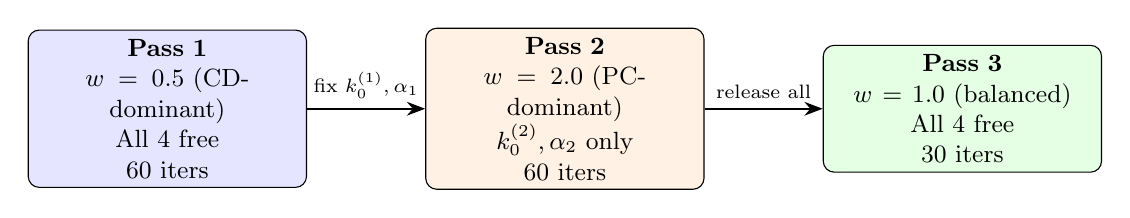
\begin{tikzpicture}[
  node distance=1.5cm,
  pass/.style={draw, rounded corners, minimum width=3.5cm, minimum height=1.4cm,
    font=\small, text width=3.3cm, align=center},
  arrow/.style={->, >=Stealth, thick},
]
  \node[pass, fill=blue!10] (p1) {
    \textbf{Pass 1}\\
    $w = 0.5$ (CD-dominant)\\
    All 4 free\\
    60 iters
  };
  \node[pass, fill=orange!10, right=of p1] (p2) {
    \textbf{Pass 2}\\
    $w = 2.0$ (PC-dominant)\\
    $\kzero^{(2)}, \alpha_2$ only\\
    60 iters
  };
  \node[pass, fill=green!10, right=of p2] (p3) {
    \textbf{Pass 3}\\
    $w = 1.0$ (balanced)\\
    All 4 free\\
    30 iters
  };

  \draw[arrow] (p1) -- node[above, font=\scriptsize] {fix $\kzero^{(1)}, \alpha_1$} (p2);
  \draw[arrow] (p2) -- node[above, font=\scriptsize] {release all} (p3);
\end{tikzpicture}
\caption{Cascade three-pass strategy. Pass~1 (CD-dominant) primarily
  recovers $\kzero^{(1)}$ and $\alpha_1$. Pass~2 (PC-dominant) focuses
  on $\kzero^{(2)}$ and $\alpha_2$ with reaction~1 parameters fixed.
  Pass~3 performs a balanced joint polish.}
\label{fig:cascade}
\end{figure}

\paragraph{Rationale.}
When $w < 1$, the objective is dominated by total current density
(sensitive to $\kzero^{(1)}$). When $w > 1$, peroxide current
(sensitive to $\kzero^{(2)}$) is emphasized. By solving sequentially
with increasing $w$, we first pin down reaction~1 parameters, then
refine reaction~2 parameters against the peroxide signal, and finally
polish all four jointly.

\subsection{Phase S4: MultiStart Grid Search}\label{sec:multistart}

\paragraph{Purpose.} Verify global optimality of the surrogate landscape
and guard against local minima.

\paragraph{Method.}
\begin{enumerate}
  \item Generate 20,000 LHS samples in the 4D parameter space (rate
    constants in log-space, transfer coefficients in linear space).
  \item Evaluate all samples via vectorized batch prediction.
  \item Select the top 20 candidates by objective value.
  \item Polish each candidate with L-BFGS-B (60 iterations).
  \item Return the best polished result.
\end{enumerate}

\paragraph{Finding.} All three strategies (S2, S3, S4) converge to the
same optimum, confirming that the NN ensemble surrogate landscape has a
\emph{single global basin}. The multi-start adds a global optimality
certificate but no accuracy improvement over S2.

\subsection{Phase S5: Best-of Selection}\label{sec:S5}

Compare the surrogate objective values from S2, S3, and S4; select the
winner. In our experiments, S4 (multi-start) achieves the marginally
lowest loss ($5.866 \times 10^{-5}$), though all three agree to 5
significant figures.

The ensemble uncertainty at the selected point is computed:
mean CD standard deviation $\sigma_{\mathrm{CD}} = 1.96 \times 10^{-4}$
and mean PC standard deviation $\sigma_{\mathrm{PC}} = 9.78 \times 10^{-4}$.
The $5\times$ higher PC uncertainty reflects the ensemble's disagreement
on the cancellation-sensitive peroxide observable and foreshadows the
difficulty of recovering $\kzero^{(2)}$.

\subsection{Phases P1--P2: PDE Refinement}\label{sec:PDE_phases}

The surrogate optimum (S5 output) is used to warm-start two PDE-constrained
optimization phases.

\paragraph{Phase P1: Shallow cathodic (10 voltage points).}
L-BFGS-B optimization with adjoint gradients on a voltage range
covering moderate cathodic overpotentials. The reduced voltage range
limits cost (\SI{104}{\second}) while providing PDE-quality gradients that
correct surrogate biases.

P1 serves primarily as a \emph{basin selector}: it ensures the optimizer
is in the correct region of parameter space before the expensive P2
phase. Ablation studies (\cref{sec:ablation}) show that skipping P1
leads to $3.2\times$ worse maximum error.

\paragraph{Phase P2: Full cathodic (15 voltage points).}
The final phase extends the voltage range to include deep cathodic
overpotentials where the peroxide current provides maximal information
about $\kzero^{(2)}$. Starting from the P1 result, L-BFGS-B converges
in 15 iterations (of a 20-iteration budget), requiring \SI{353}{\second}.

\emph{Key mechanism.} At deep cathodic potentials, both reactions are
strongly driven, and the ratio $\mathcal{R}_1/\mathcal{R}_2$ becomes
more sensitive to $\kzero^{(2)}$. The PDE's exact treatment of this
ratio---unavailable to the surrogate's approximate function---enables P2
to break the $\kzero^{(1)}$--$\kzero^{(2)}$ anti-correlation and reduce
$\kzero^{(2)}$ error from $12\%$ (surrogate) to $4.2\%$.

\begin{algorithm}[H]
\DontPrintSemicolon
\caption{v13 Inference Pipeline}\label{alg:pipeline}
\KwIn{Observed I--V curves $I_{\mathrm{CD}}^{\mathrm{obs}}$,
  $I_{\mathrm{PC}}^{\mathrm{obs}}$; trained NN ensemble $\mathcal{E}$;
  PDE forward solver $\mathcal{F}$}
\KwOut{Estimated parameters $\hat{\vect{\theta}}$}

\BlankLine
\tcc{Surrogate tier}
$\vect{\theta}_0 \gets \text{cold guess}$\;
$\alpha_1^*, \alpha_2^* \gets \textsc{S1-AlphaInit}(\vect{\theta}_0, \mathcal{E})$\;
$\vect{\theta}_{\text{S2}} \gets \textsc{S2-JointLBFGSB}(\vect{\theta}_0[\alpha\!\gets\!\alpha^*], \mathcal{E})$\;
$\vect{\theta}_{\text{S3}} \gets \textsc{S3-Cascade}(\vect{\theta}_{\text{S2}}, \mathcal{E})$\;
$\vect{\theta}_{\text{S4}} \gets \textsc{S4-MultiStart}(\mathcal{E})$\;
$\vect{\theta}_{\text{S5}} \gets \argmin_{\vect{\theta} \in \{\vect{\theta}_{\text{S2}}, \vect{\theta}_{\text{S3}}, \vect{\theta}_{\text{S4}}\}} \Jobj_{\mathcal{E}}(\vect{\theta})$\;

\BlankLine
\tcc{PDE tier}
$\vect{\theta}_{\text{P1}} \gets \textsc{P1-PDE-Shallow}(\vect{\theta}_{\text{S5}}, \mathcal{F}, \eta_{\text{shallow}})$\;
$\hat{\vect{\theta}} \gets \textsc{P2-PDE-Full}(\vect{\theta}_{\text{P1}}, \mathcal{F}, \eta_{\text{full}})$\;
\Return $\hat{\vect{\theta}}$\;
\end{algorithm}

%==========================================================================
\section{Results}\label{sec:results}
%==========================================================================

All results use synthetic observations generated from the true parameters
(\cref{tab:constants}) with $2\%$ additive Gaussian noise (seed 20260226).
\Cref{fig:iv_curves} shows the forward model I--V curves at the true
parameter values, illustrating the two observables that the inverse
problem seeks to match.

\begin{figure}[H]
\centering
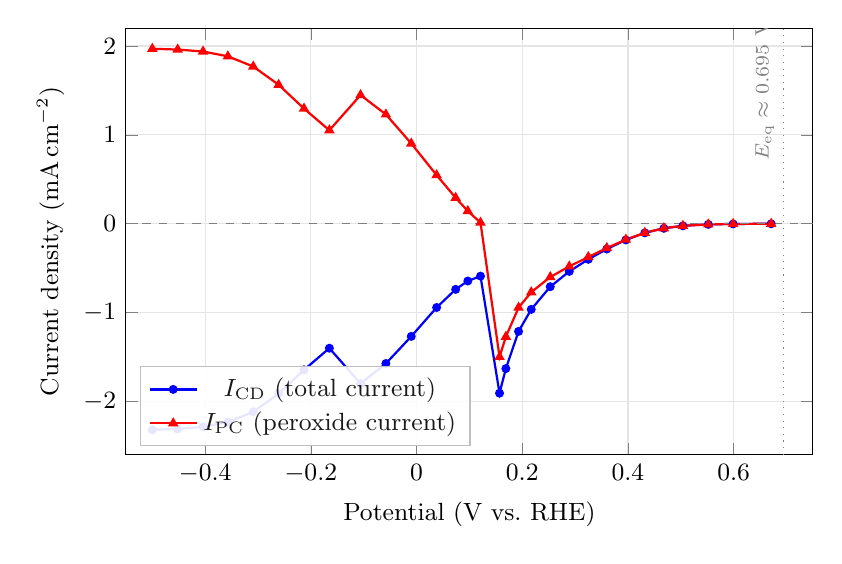
\begin{tikzpicture}
\begin{axis}[
  width=0.85\textwidth,
  height=7cm,
  xlabel={Potential (V vs.\ RHE)},
  ylabel={Current density (\si{\milli\ampere\per\centi\metre\squared})},
  xmin=-0.55, xmax=0.75,
  ymin=-2.6, ymax=2.2,
  grid=major,
  grid style={gray!20},
  legend style={at={(0.02,0.02)}, anchor=south west, font=\small,
    fill=white, fill opacity=0.9, draw=gray!50},
  every axis plot/.append style={thick},
  tick label style={font=\small},
  label style={font=\small},
]
% Total current density (I_CD) — from bv_iv_curve.csv
\addplot[blue, mark=*, mark size=1.2pt] coordinates {
  (-0.500, -2.317) (-0.452, -2.308) (-0.404, -2.285)
  (-0.357, -2.231) (-0.309, -2.116) (-0.261, -1.911)
  (-0.213, -1.644) (-0.165, -1.400)
  (-0.106, -1.798) (-0.058, -1.572)
  (-0.010, -1.267)
  (0.038, -0.942) (0.074, -0.738) (0.097, -0.644)
  (0.121, -0.589) (0.157, -1.906) (0.169, -1.629)
  (0.193, -1.211) (0.217, -0.963)
  (0.253, -0.708) (0.289, -0.536) (0.325, -0.400)
  (0.360, -0.284) (0.396, -0.182) (0.432, -0.102)
  (0.468, -0.051) (0.504, -0.023) (0.552, -0.007)
  (0.599, -0.002) (0.671, 0.000)
};
\addlegendentry{$I_{\mathrm{CD}}$ (total current)}

% Peroxide current density (I_PC) — from bv_iv_curve.csv
\addplot[red, mark=triangle*, mark size=1.4pt] coordinates {
  (-0.500, 1.969) (-0.452, 1.960) (-0.404, 1.938)
  (-0.357, 1.884) (-0.309, 1.769) (-0.261, 1.564)
  (-0.213, 1.296) (-0.165, 1.052)
  (-0.106, 1.448) (-0.058, 1.230)
  (-0.010, 0.903)
  (0.038, 0.547) (0.074, 0.292) (0.097, 0.143)
  (0.121, 0.013) (0.157, -1.498) (0.169, -1.271)
  (0.193, -0.943) (0.217, -0.770)
  (0.253, -0.599) (0.289, -0.480) (0.325, -0.374)
  (0.360, -0.273) (0.396, -0.178) (0.432, -0.101)
  (0.468, -0.050) (0.504, -0.023) (0.552, -0.007)
  (0.599, -0.002) (0.671, 0.000)
};
\addlegendentry{$I_{\mathrm{PC}}$ (peroxide current)}

% Zero line
\draw[gray, thin, dashed] (axis cs:-0.55,0) -- (axis cs:0.75,0);

% Equilibrium annotation
\draw[gray, thin, dotted] (axis cs:0.695,-2.6) -- (axis cs:0.695,2.2);
\node[gray, font=\scriptsize, rotate=90, anchor=south] at (axis cs:0.695,1.5)
  {$E_{\mathrm{eq}} \approx 0.695$ V};

\end{axis}
\end{tikzpicture}
\caption{Forward model I--V curves at the true parameter values
  ($\kzero^{(1)} = 2.4\times10^{-8}$~m/s,
   $\kzero^{(2)} = 1.0\times10^{-9}$~m/s,
   $\alpha_1 = 0.627$, $\alpha_2 = 0.5$).
  Blue: total current density $I_{\mathrm{CD}}$ (analogous to disk
  current in RRDE). Red: peroxide current density $I_{\mathrm{PC}}$
  (analogous to ring current). Near equilibrium ($\sim\!0.7$~V vs.\ RHE)
  both currents vanish; at cathodic potentials the total current
  approaches the diffusion-limited plateau while the peroxide current
  reflects the competition between R$_1$ (production) and R$_2$
  (consumption). The non-monotonic feature in $I_{\mathrm{PC}}$ near
  $0.1$--$0.15$~V arises from the transition where R$_2$ begins to
  dominate peroxide consumption.}
\label{fig:iv_curves}
\end{figure}

\subsection{Surrogate Phase Results}\label{sec:surr_results}

\begin{table}[H]
\centering
\caption{Surrogate phase results (S1--S5). All percentage errors are
  relative to true parameter values.}
\label{tab:surr_results}
\begin{tabular}{llrrrrc}
\toprule
Phase & Strategy & $\kzero^{(1)}$ & $\kzero^{(2)}$ & $\alpha_1$ & $\alpha_2$ & Max \\
\midrule
S1 & Alpha-only init   & 49.7\%  & 78.5\%  & 49.7\% & 78.5\% & 78.5\% \\
S2 & Joint L-BFGS-B    &  6.88\% & 11.85\% & 3.54\% & 3.48\% & 11.85\% \\
S3 & Cascade 3-pass    &  6.89\% & 12.24\% & 3.57\% & 3.43\% & 12.24\% \\
S4 & MultiStart 20K    &  6.89\% & 12.05\% & 3.55\% & 3.44\% & 12.05\% \\
\midrule
\textbf{S5} & \textbf{Best (S4)} & \textbf{6.89\%} & \textbf{12.05\%}
  & \textbf{3.55\%} & \textbf{3.44\%} & \textbf{12.05\%} \\
\bottomrule
\end{tabular}
\end{table}

\paragraph{Key finding.}
All three optimization strategies converge to essentially the same
optimum (losses agree to 5 significant figures). This confirms a
\emph{single global basin} in the NN ensemble surrogate landscape.
The cascade and multi-start add robustness (a global optimality
certificate) but not accuracy. The surrogate plateau at
$\sim\!12\%$ $\kzero^{(2)}$ error represents the fundamental resolution
limit of the NN approximation on this observable.

\subsection{PDE Phase Results}\label{sec:pde_results}

\begin{table}[H]
\centering
\caption{PDE refinement results (P1--P2).}
\label{tab:pde_results}
\begin{tabular}{llrrrrc}
\toprule
Phase & Grid & $\kzero^{(1)}$ & $\kzero^{(2)}$ & $\alpha_1$ & $\alpha_2$ & Max \\
\midrule
P1 & Shallow (10 pts) & 6.80\% & 12.01\% & 3.88\% & 3.17\% & 12.01\% \\
\textbf{P2} & \textbf{Full (15 pts)} & \textbf{4.78\%} & \textbf{4.23\%}
  & \textbf{2.95\%} & \textbf{5.26\%} & \textbf{5.26\%} \\
\bottomrule
\end{tabular}
\end{table}

\paragraph{The P2 breakthrough.}
The transition from P1 to P2 produces the paper's central result:
$\kzero^{(2)}$ error drops from $12.0\%$ to $4.23\%$---a $2.8\times$
improvement. The extended voltage range provides deep-cathodic peroxide
current data where Reaction~2 makes a non-negligible contribution,
enabling the PDE solver to resolve the $\kzero^{(1)}$--$\kzero^{(2)}$
degeneracy.

\paragraph{Redimensionalized values.}
\begin{center}
\begin{tabular}{lccc}
\toprule
Parameter & True & Estimated & Error \\
\midrule
$\kzero^{(1)}$ & $2.400\times10^{-8}$ m/s & $2.515\times10^{-8}$ m/s & 4.78\% \\
$\kzero^{(2)}$ & $1.000\times10^{-9}$ m/s & $9.577\times10^{-10}$ m/s & 4.23\% \\
$\alpha_1$ & 0.627 & 0.609 & 2.95\% \\
$\alpha_2$ & 0.500 & 0.474 & 5.26\% \\
\bottomrule
\end{tabular}
\end{center}

\subsection{Historical Comparison}\label{sec:history}

\begin{table}[H]
\centering
\caption{Cross-version comparison of inference results at $2\%$ noise.}
\label{tab:history}
\begin{tabular}{llrrrrc}
\toprule
Version & Architecture & $\kzero^{(1)}$ & $\kzero^{(2)}$ & $\alpha_1$
  & $\alpha_2$ & Max \\
\midrule
v7  & PDE only       & 10.9\% & 2.6\%  & 5.6\% & 8.8\%  & 10.9\% \\
v9  & RBF surrogate  & 8.8\%  & 7.6\%  & 4.8\% & 6.4\%  & 8.8\% \\
v11 & RBF$\to$PDE    & 9.4\%  & 0.8\%  & 5.1\% & 7.8\%  & 9.4\% \\
v12 & NN$\to$PDE     & 6.8\%  & 11.8\% & 3.9\% & 3.2\%  & 11.8\% \\
\midrule
\textbf{v13} & \textbf{NN (multi)$\to$PDE} & \textbf{4.78\%} & \textbf{4.23\%}
  & \textbf{2.95\%} & \textbf{5.26\%} & \textbf{5.26\%} \\
\bottomrule
\end{tabular}
\end{table}

v13 is the first version to achieve $< 10\%$ error on all four
parameters simultaneously, and the first to break the
$\kzero^{(1)}$--$\kzero^{(2)}$ trade-off (lowest sum at $9.01\%$ and
lowest max at $5.26\%$).

\subsection{Ablation: Skip-P1}\label{sec:ablation}

To assess whether Phase P1 is essential, we run an ablation that skips
P1 and feeds the surrogate result (S5) directly to P2.

\begin{table}[H]
\centering
\caption{Ablation: effect of skipping Phase P1.}
\label{tab:ablation}
\begin{tabular}{lcc}
\toprule
Metric & v13 (with P1) & v13 (skip P1) \\
\midrule
$\kzero^{(1)}$ error  & 4.78\%   & 16.99\% \\
$\kzero^{(2)}$ error  & 4.23\%   & 6.15\% \\
$\alpha_1$ error       & 2.95\%   & 8.24\% \\
$\alpha_2$ error       & 5.26\%   & 11.78\% \\
\midrule
Max error              & \textbf{5.26\%} & 16.99\% \\
P2 time                & 353s     & 469s \\
Total time             & 541s     & 552s \\
\bottomrule
\end{tabular}
\end{table}

Skipping P1 degrades all parameters and makes P2 paradoxically
\emph{slower} (the optimizer starts further from the PDE basin and
requires more forward solves). P1 is not redundant; it is an essential
basin selector.

\subsection{Timing Breakdown}\label{sec:timing}

\begin{table}[H]
\centering
\caption{Wall-clock timing breakdown for the v13 pipeline.}
\label{tab:timing}
\begin{tabular}{lrr}
\toprule
Stage & Time (s) & Fraction \\
\midrule
Target generation (PDE at truth) & 71.7 & 13.3\% \\
S1: Alpha-only init & 0.1 & $<0.1\%$ \\
S2: Joint L-BFGS-B & 0.6 & 0.1\% \\
S3: Cascade (3 passes) & 1.0 & 0.2\% \\
S4: MultiStart (20K + polish) & 9.8 & 1.8\% \\
\midrule
P1: PDE shallow cathodic & 103.9 & 19.2\% \\
P2: PDE full cathodic & 353.3 & 65.3\% \\
\midrule
\textbf{Total} & \textbf{540.9} & \textbf{100\%} \\
\bottomrule
\end{tabular}
\end{table}

Surrogate phases S1--S4 collectively cost \SI{11.5}{\second} ($2.1\%$ of
total), while PDE phases account for $84.5\%$. The surrogate's role is
\emph{warm-starting}, not accuracy: it provides a good initial guess that
reduces PDE optimization cost by $\sim\!30\%$ compared to cold starts.


%==========================================================================
\section{Computational Optimizations}\label{sec:optimizations}
%==========================================================================

\subsection{Parallel PDE Evaluation}\label{sec:parallel}

Each PDE phase requires evaluating the forward model at multiple voltage
points. These evaluations are independent and can be parallelized using a
process-based worker pool:
\begin{itemize}
  \item Pool size: $\min(M, \texttt{cpu\_count} - 1)$, where $M$ is the
    number of voltage points.
  \item Workers are spawned via Python's \texttt{multiprocessing} module.
  \item Each worker imports Firedrake independently (no shared state).
  \item Results are gathered and assembled into I--V curves.
\end{itemize}

\subsection{IC Cache and Warm-Starting}\label{sec:cache}

Warm-starting is the single most impactful optimization. Two cache levels
are maintained:
\begin{enumerate}
  \item \textbf{All-points cache:} Stores converged solutions for every
    $(k_0, \alpha, \eta)$ triple evaluated during optimization. Subsequent
    evaluations at the same $\eta$ with nearby parameters start from the
    cached solution.
  \item \textbf{Cross-evaluation cache:} Solutions from evaluation $n$
    warm-start evaluation $n+1$, exploiting the fact that L-BFGS-B
    steps are small in parameter space.
\end{enumerate}
Warm-started solves use \texttt{max\_steps=20} pseudo-transient iterations,
versus 50--100 for cold starts. This reduces per-evaluation cost by
$\sim\!60\%$.

\subsection{Two-Tape Adjoint}\label{sec:two_tape}

The multi-observable objective \eqref{eq:objective} requires derivatives
with respect to both $I_{\mathrm{CD}}$ and $I_{\mathrm{PC}}$. Rather than
two forward solves (one taped per observable), we use a single forward
solve with two adjoint passes:
\begin{enumerate}
  \item Tape the forward solve once.
  \item Adjoint pass 1: differentiate $I_{\mathrm{CD}}$ w.r.t.\
    $\vect{\theta}$ $\to$ $\nabla_{\vect{\theta}} J_{\mathrm{CD}}$.
  \item Adjoint pass 2: differentiate $I_{\mathrm{PC}}$ w.r.t.\
    $\vect{\theta}$ $\to$ $\nabla_{\vect{\theta}} J_{\mathrm{PC}}$.
  \item Combine: $\nabla \Jobj = \nabla J_{\mathrm{CD}} + w\,\nabla J_{\mathrm{PC}}$.
\end{enumerate}
This halves the forward computation cost relative to a naive implementation.

\subsection{Shared Pool Reuse}\label{sec:pool_reuse}

The worker pool is created once at the start of P1 and reused for P2.
This saves $\sim\!\SI{10}{\second}$ of Firedrake import overhead per
worker. Between phases, the solution cache is cleared to prevent stale
warm-starts from misguiding the optimizer.


%==========================================================================
\section{Discussion}\label{sec:discussion}
%==========================================================================

\subsection{Why \texorpdfstring{$k_{0,2}$}{k0,2} Is the Bottleneck}

The difficulty of recovering $\kzero^{(2)}$ has three layers:

\paragraph{Physical.} At moderate overpotentials ($|\eta| < \SI{0.5}{\volt}$),
Reaction~2's rate is $\sim\!24\times$ smaller than Reaction~1's. The
total current is insensitive to $\kzero^{(2)}$, and the peroxide current
$I_{\mathrm{PC}} = I_{\mathrm{R1}} - I_{\mathrm{R2}}$ is a difference
of two nearly equal quantities---amplifying measurement noise.

\paragraph{Surrogate.} The NN ensemble's uncertainty on peroxide current
($\sigma_{\mathrm{PC}} = 9.78 \times 10^{-4}$) is $5\times$ higher than
on current density ($\sigma_{\mathrm{CD}} = 1.96 \times 10^{-4}$). The
ensemble members disagree most where the signal-to-noise ratio is worst.
This places a fundamental floor on surrogate-only recovery of $\kzero^{(2)}$.

\paragraph{Voltage range.} At deep cathodic potentials, both reactions
saturate and $I_{\mathrm{PC}}$ becomes more sensitive to $\kzero^{(2)}$.
The transition from P1 (shallow) to P2 (full cathodic) provides exactly
this information, enabling the $12\% \to 4.2\%$ breakthrough.

\subsection{The Continuation Analogy}\label{sec:cont_analogy}

The P1$\to$P2 transition can be understood as a continuation method in
parameter space. P1 solves an \emph{easier problem} (fewer voltage
points, reduced landscape complexity) that nonetheless constrains the
solution to a basin near the global optimum. P2 then refines within this
basin using richer data.

This is analogous to classical homotopy methods in nonlinear optimization,
where a sequence of problems $\Jobj_\lambda$ ($\lambda \in [0,1]$)
interpolates between a tractable proxy and the true objective. Here,
$\lambda$ is implicitly controlled by the voltage range: more data
$\Rightarrow$ harder but more informative problem.

The ablation (\cref{tab:ablation}) quantifies the cost of skipping this
continuation: without P1, P2 converges to a worse local minimum with
$3.2\times$ higher maximum error.

\subsection{Surrogate vs.\ PDE Roles}\label{sec:roles}

The pipeline embodies a \emph{multi-fidelity paradigm}:
\begin{itemize}
  \item \textbf{Surrogates for exploration:} Fast ($\SI{1}{\milli\second}$
    per evaluation), approximate, used to identify the global basin and
    provide warm-starts. Three independent strategies confirm global
    optimality.
  \item \textbf{PDE for refinement:} Slow ($\SI{20}{\second}$ per
    evaluation), exact, used for final parameter recovery where surrogate
    accuracy is insufficient (particularly for $\kzero^{(2)}$).
\end{itemize}

The surrogate phases contribute only $2\%$ of total cost yet are
essential: without them, PDE phases would require cold starts and
potentially converge to inferior local minima.

\subsection{Limitations}\label{sec:limitations}

Several limitations should be noted:
\begin{enumerate}
  \item \textbf{Single noise seed:} Results are reported for one noise
    realization (seed 20260226). Robustness across noise seeds has not
    been verified.
  \item \textbf{Specific geometry:} The 2D rectangle with $L_{\mathrm{ref}}
    = \SI{100}{\micro\metre}$ is specific to the RDE configuration.
    Extension to 3D or different geometries requires retraining surrogates.
  \item \textbf{Noise level:} Only $2\%$ Gaussian noise has been tested.
    At $0\%$ noise, v11 achieved $1.07\%$ maximum error, suggesting that
    noise is the dominant error source---a $9\times$ degradation.
  \item \textbf{Surrogate training cost:} The $\sim\!2000$ PDE solves for
    training data generation ($\sim\!\SI{10}{\hour}$) are a one-time cost
    not included in the pipeline timing.
\end{enumerate}


%==========================================================================
\section{Conclusions}\label{sec:conclusions}
%==========================================================================

We presented a seven-phase multi-fidelity inference pipeline that
recovers four Butler--Volmer kinetic parameters from noisy I--V curve
measurements with $< 5.3\%$ maximum error. The key results are:

\begin{enumerate}
  \item \textbf{Breaking the trade-off:} v13 is the first pipeline version
    to achieve $< 10\%$ error on all four parameters simultaneously,
    resolving the persistent $\kzero^{(1)}$--$\kzero^{(2)}$
    anti-correlation that limited prior versions.
  \item \textbf{Multi-fidelity architecture:} The combination of NN
    ensemble surrogates (for global exploration) with PDE-constrained
    optimization (for local refinement) is more effective than either
    approach alone. Surrogates provide basin identification at $2\%$ of
    total cost; PDE phases provide the accuracy.
  \item \textbf{Continuation is essential:} The shallow-voltage PDE phase
    (P1) serves as a basin selector for the full-cathodic phase (P2).
    Skipping P1 degrades maximum error by $3.2\times$.
  \item \textbf{Voltage range matters:} Deep cathodic overpotentials
    provide the peroxide current signal needed to resolve $\kzero^{(2)}$,
    explaining the $12\% \to 4.2\%$ improvement from P1 to P2.
\end{enumerate}

Future work includes noise robustness studies across multiple noise
seeds, exploration of alternative surrogate architectures (e.g.,
physics-informed neural operators), and extension to three-dimensional
electrode geometries.


%==========================================================================
% Bibliography (inline for self-containment)
%==========================================================================
\begin{thebibliography}{9}

\bibitem{mangan2025}
N.~M.~Mangan \emph{et al.},
``Mathematical Investigation of Bulk and Local Effects in Electrocatalysis,''
Northwestern University, 2025.

\bibitem{ruggiero2022}
B.~Ruggiero, L.~Seitz \emph{et al.},
``pH Effects on Oxygen Reduction Catalysis on Carbon-Supported Catalysts,''
\emph{J.\ Catalysis}, vol.~414, pp.~33--43, 2022.

\bibitem{firedrake}
F.~Rathgeber \emph{et al.},
``Firedrake: automating the finite element method by composing abstractions,''
\emph{ACM Trans.\ Math.\ Softw.}, vol.~43, no.~3, 2016.

\bibitem{pyadjoint}
S.~W.~Funke and P.~E.~Farrell,
``A framework for automated PDE-constrained optimisation,''
\emph{arXiv:1302.3894}, 2013.

\bibitem{petsc}
S.~Balay \emph{et al.},
``PETSc Users Manual,'' Argonne National Laboratory, Tech.~Rep.
ANL-95/11---Rev.~3.18, 2022.

\bibitem{lbfgsb}
R.~H.~Byrd, P.~Lu, J.~Nocedal, and C.~Zhu,
``A limited memory algorithm for bound constrained optimization,''
\emph{SIAM J.\ Sci.\ Comput.}, vol.~16, no.~5, pp.~1190--1208, 1995.

\bibitem{adamw}
I.~Loshchilov and F.~Hutter,
``Decoupled weight decay regularization,''
in \emph{ICLR}, 2019.

\bibitem{lhs}
M.~D.~McKay, R.~J.~Beckman, and W.~J.~Conover,
``A comparison of three methods for selecting values of input variables
in the analysis of output from a computer code,''
\emph{Technometrics}, vol.~21, no.~2, pp.~239--245, 1979.

\bibitem{mumps}
P.~R.~Amestoy, I.~S.~Duff, J.-Y.~L'Excellent, and J.~Koster,
``A fully asynchronous multifrontal solver using distributed dynamic scheduling,''
\emph{SIAM J.\ Matrix Anal.\ Appl.}, vol.~23, no.~1, pp.~15--41, 2001.

\bibitem{SER}
W.~Mulder and B.~van Leer,
``Experiments with implicit upwind methods for the Euler equations,''
\emph{J.\ Comput.\ Phys.}, vol.~59, pp.~232--246, 1985.

\end{thebibliography}

\end{document}
